All datasets were spatially harmonized using a common grid resolution of $0.1^\circ \times 0.1^\circ$. 
The merging process was performed incrementally, combining datasets two by two based on spatial correspondence.

First, the fire dataset was merged with the land cover dataset using a spatial join based on geographic location. 
Each fire detection point was assigned to a grid cell represented as a polygon. 
A match was established when the fire point fell inside the corresponding land cover polygon.

Subsequently, additional environmental datasets, including elevation, climate, and soil data, were merged using the same grid-cell polygons as the spatial reference. 
Since these datasets were already represented at the grid level, the merging was performed directly through polygon-based matching rather than point-in-polygon operations.

This polygon-based integration ensured spatial consistency across all variables and allowed all datasets to be aligned to a unified spatial resolution, facilitating subsequent feature engineering and modeling.

\begin{figure}[H]
    \centering
    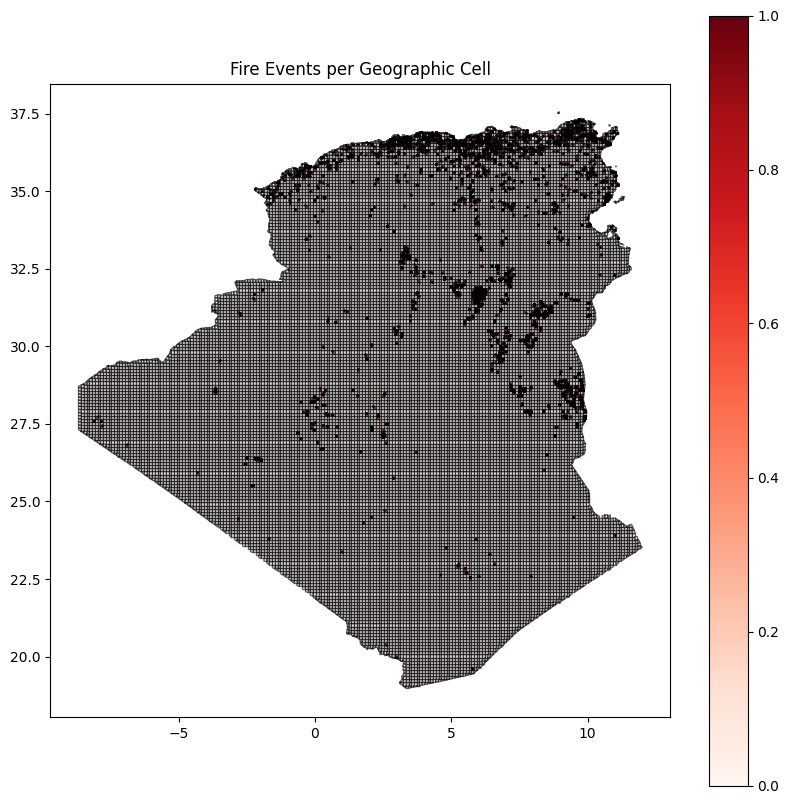
\includegraphics[width=0.35\textwidth]{images/MergedDatasetsImages/fire_events per geographical cell.png}
    \caption{Distribution of fire events aggregated per $0.1^\circ \times 0.1^\circ$ geographical grid cell}
\end{figure}


\begin{itemize}
    \item \textbf{Centroid-based merging:} Climate and soil polygons were matched using representative points (centroids). Exact matches were prioritized, and unmatched climate points were linked to the nearest soil polygon.
    % \item \textbf{Column dropping:} To simplify the dataset, several redundant or internal-use columns were removed, including \texttt{geometry}, \texttt{cell\_id}, \texttt{match\_type}, \texttt{distance\_m}, \texttt{area\_log}, \texttt{x}, and \texttt{y}.
    % \item \textbf{Elevation addition:} Elevation values were sampled from a raster at the coordinates of the merged polygons and added as a new column.
    % \item \textbf{Resulting dataset:} After dropping these columns, the dataset retains only the necessary features for further analysis, while internal identifiers and duplicate coordinates are removed.
    \item \textbf{Visualization:} Coverage maps for climate and soil polygons, as well as elevation distributions and spatial maps, were generated to assess data completeness and spatial consistency.
\end{itemize}

\begin{figure}[H]
    \centering
    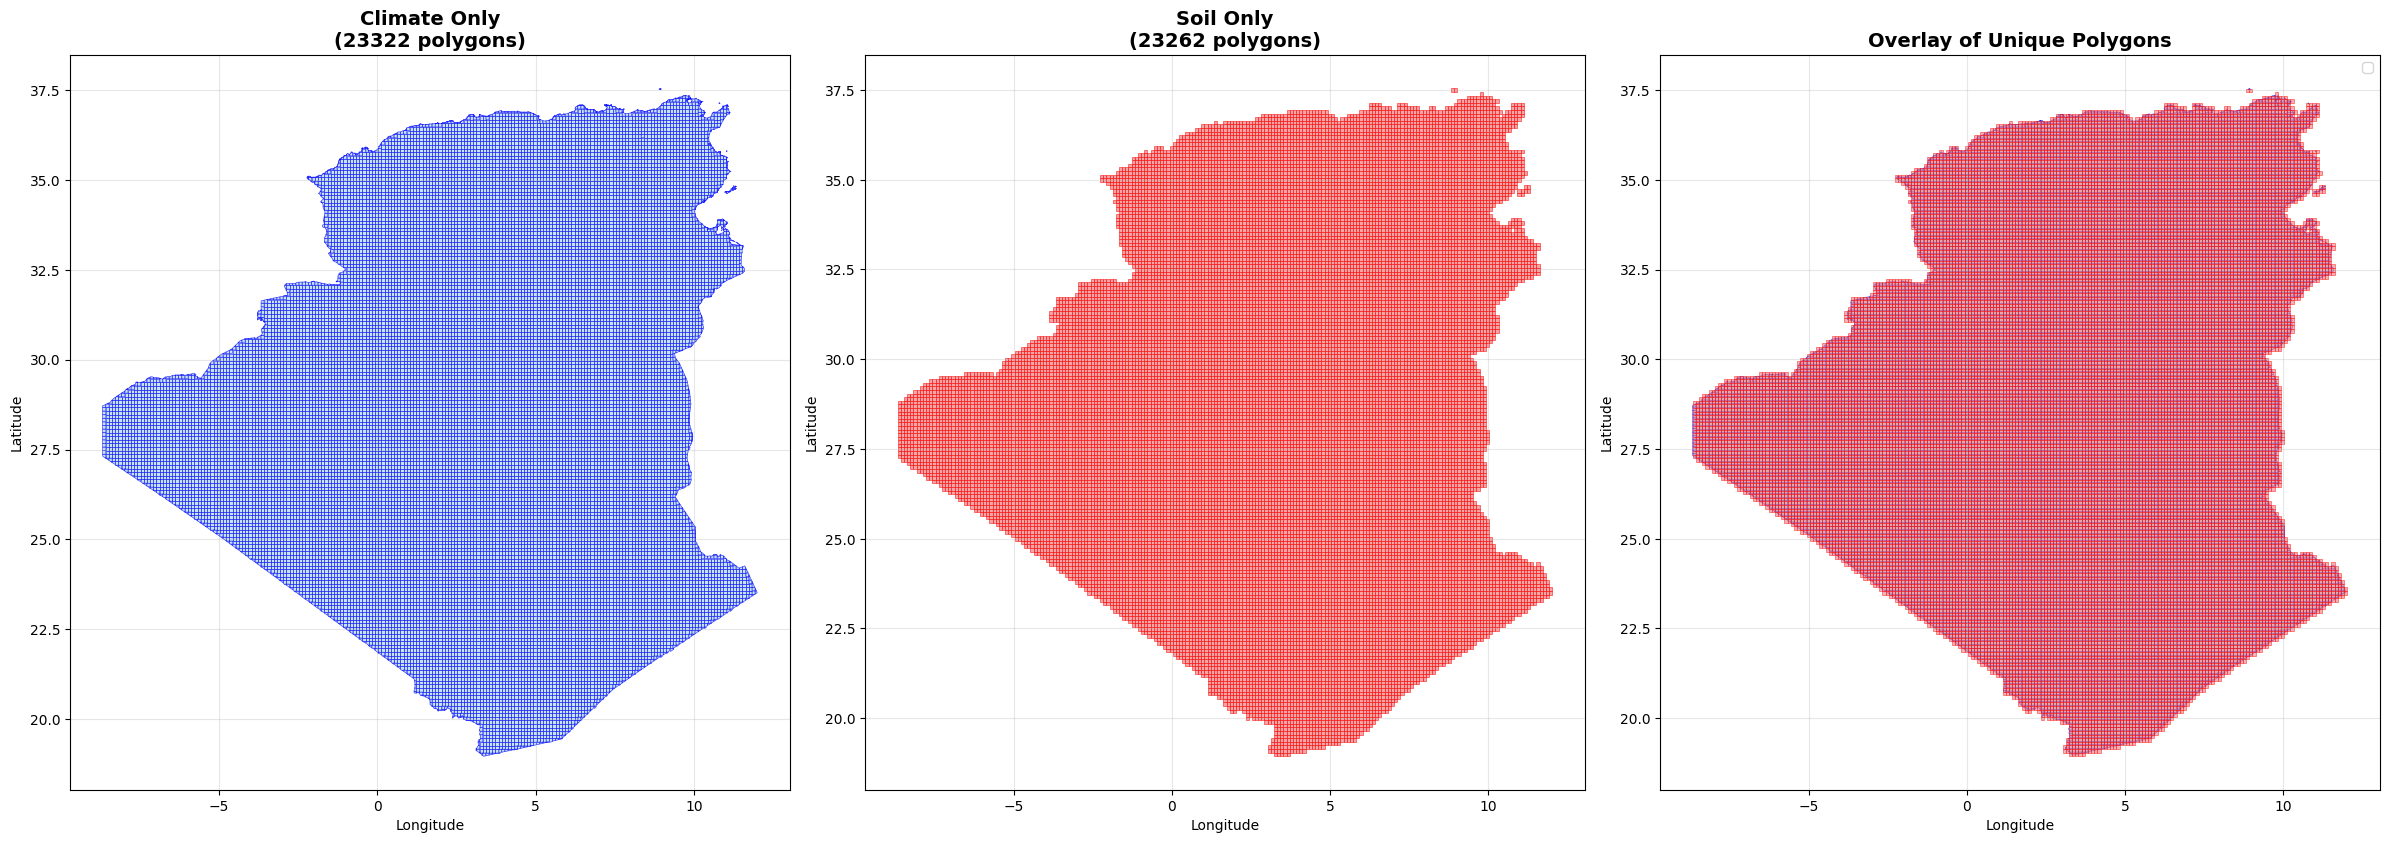
\includegraphics[width=0.8\textwidth]{images/MergedDatasetsImages/climate_soil_coverage.png}
    \caption{Coverage of climate (blue) and soil (red) polygons. Coverage of merged (pink)}
    \label{fig:merge_overview}
\end{figure}
